\documentclass{article}
\usepackage[greek]{babel}
\usepackage[utf8]{inputenc}
\usepackage{johd}
\usepackage{graphicx}
\usepackage{gensymb}
\usepackage{amsmath}
\usepackage{booktabs}
\usepackage{indentfirst}
\usepackage{hyperref}

\title{\textlatin{AD\_Pend\_4}}

\author{\textlatin{Anastasios-Faidon Retselis (AEM: 4394)}}
\date{9/5/2021}

\begin{document}
\maketitle

Εξετάζεται η περίπτωση 4, οπότε οι παράμετροι είναι: 

\begin{equation}
    f=sin,\; \omega=3,\; \epsilon=0.1 
\end{equation}

\section{Άσκηση}

\indent Έστω εκκρεμές το οποίο του μετβάλλουμε το μήκος περιοδικά:

\begin{equation}
\ddot{\theta}=-\frac{g}{l} \sin \theta
\end{equation}

όπου:

\begin{equation}
l=l_{0}+\varepsilon f(\omega t)
\end{equation}

όπου \textlatin{f} είναι μια περιοδική συνάρτηση πλάτους 1 και γωνιακής συχνότητας \(\omega\) και \(\epsilon << l_{0}\).


\subsection{Ερώτημα Α}

\indent Γράψτε τη ΔΕ ως ενα ταλαντωτή στη μορφή:

\begin{equation}
\ddot{\theta}=f(\theta)+\varepsilon g(\theta, t)+O\left(\varepsilon^{2}\right)
\end{equation}

\subsubsection{Λύση}

\indent H (2) γράφεται στη μορφή:

\begin{align}
    \ddot{\theta} &=-\frac{g}{(l_{0}+\epsilon f(\omega, t))} \sin \theta \\
    \Rightarrow \ddot{\theta} &=-\frac{g}{l_{0}(1+\frac{\epsilon f(\omega, t)}{l_{0}}}) \sin \theta \\
    \Rightarrow \ddot{\theta} &=-\frac{g}{l_{0}} \sin \theta \frac{1}{(1+\frac{\epsilon f(\omega, t)}{l_{0}})}
\end{align}

Όπου μπορούμε να εφαρμόσουμε ανάπτυγμα \textlatin{Taylor} για τον τελευταίο όρο και έχουμε:

\begin{align}
    \Rightarrow \ddot{\theta} &=-\frac{g}{l_{0}} \sin \theta (1-\frac{\epsilon f(\omega, t)}{l_{0}})+Ο(\epsilon^{2}) \\
    \Rightarrow \ddot{\theta} &=-\frac{g}{l_{0}} \sin \theta + \frac{\epsilon g f(\omega, t) \sin \theta}{l_{0}^2}+Ο(\epsilon^{2})
\end{align}

Σχέση η οποία είναι στην ζητούμενη μορφή της εκφώνησης.

\subsection{Ερώτημα Β}

\indent Σχεδιάστε την τομή \textlatin{Poincare} του συστήματος για τις παραμέτρους που δίνονται.

\subsubsection{Λύση}

\indent
Για την περίπτωση 4,  οι παράμετροι είναι: 

\begin{equation}
    f=sin,\; \omega=3,\; \epsilon=0.1 
\end{equation}

και επομένως η εξίσωση γίνεται:

\begin{equation}
    \ddot{\theta} =-\frac{1}{(1+0.1 \sin (3 t))} \sin \theta
\end{equation}

Θα λύσουμε την παραπάνω εξίσωση στη \textlatin{Mathematica} χρησιμοποιώντας τις ακόλουθες αρχικές συνθήκες για να πάρουμε την τομή \textlatin{Poincare}:

\begin{table}[H]
\caption{Αρχικές συνθήκες για την τομή \textlatin{Poincare}}
\centering
\begin{tabular}{|c|c|}
\hline
\(\theta(0)\)  & \(\dot{\theta}(0)\) \\ \hline
1.90845 & 0.4508    \\ \hline
0.5     & 0         \\ \hline
0.8     & 0         \\ \hline
2.0     & 0         \\ \hline
1.5     & 0.5       \\ \hline
1.0     & 0.6       \\ \hline
0.01    & 0.01      \\ \hline
2.6     & 0.2       \\ \hline
3.0     & 0.2       \\ \hline
4.0     & 0.2       \\ \hline
4.0     & 1.5       \\ \hline
4.0     & -1.5      \\ \hline
4.0     & 2.0       \\ \hline
4.0     & -2.0       \\ \hline
\end{tabular}
\end{table}

\begin{figure}[H]
    \centering
    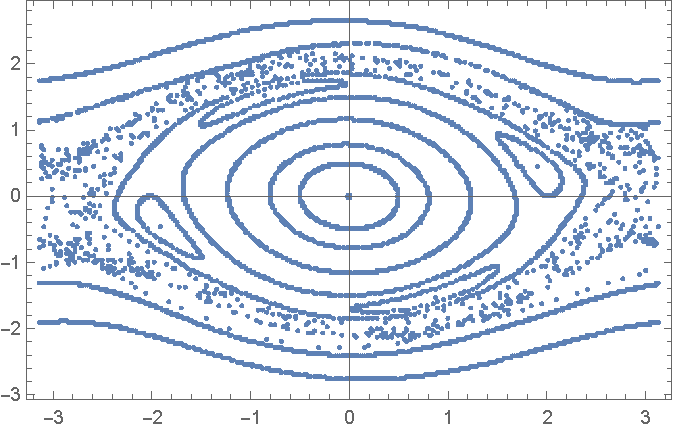
\includegraphics[]{AD_Pend_4/poincare.pdf}
    \caption{Η τομή \textlatin{Poincare} για διαφορετικές αρχικές συνθήκες}
    \label{fig:poincare_b}
\end{figure}

\subsection{Ερώτημα Γ}

\indent Εντοπίστε και δώστε αρχικές συνθήκες για μια περιοδική προσεγγιστικα τροχιά (όχι κοντά στο \(\theta = \dot{\theta} =0\)), μια ημιπεριοδική και μια χαοτική τροχιά και υπολογίστε τον δείκτη \textlatin{FLI} για την κάθε μια (σε ένα διάγραμμα και για τις τρεις τροχίες)

\subsubsection{Λύση}

\indent Οι τροχίες που επιλέχθηκαν φαίνονται στον παρακάτω πίνακα:

\begin{table}[H]
\centering
\caption{Αρχικές συνθήκες για τις τρεις ζητούμενες τροχιές}
\begin{tabular}{|c|c|c|}
\hline
\textbf{Τύπος}        & \(\theta(0)\)      & \(\dot{\theta}(0)\)  \\ \hline
Περιοδική    & 1.90845 & 0.4508 \\ \hline
Ημιπεριοδική & 0.5     & 0      \\ \hline
Χαοτική      & 2.6     & 0.2    \\ \hline
\end{tabular}
\end{table}

Αξίζει να σημειώσουμε πως η για την περιοδική τροχιά παρατηρούμε τις λεγόμενες νησίδες και πως η ευσταθής τροχιά είναι πολλαπλότητας 4. Στη συνέχεια, υπολογίζουμε ξεχωριστά τον δείκτη \textlatin{FLI} για κάθε τροχιά και συγκεντρώνουμε τα αποτελέσματα μας σε ένα διάγραμμα.

\begin{figure}[H]
    \centering
    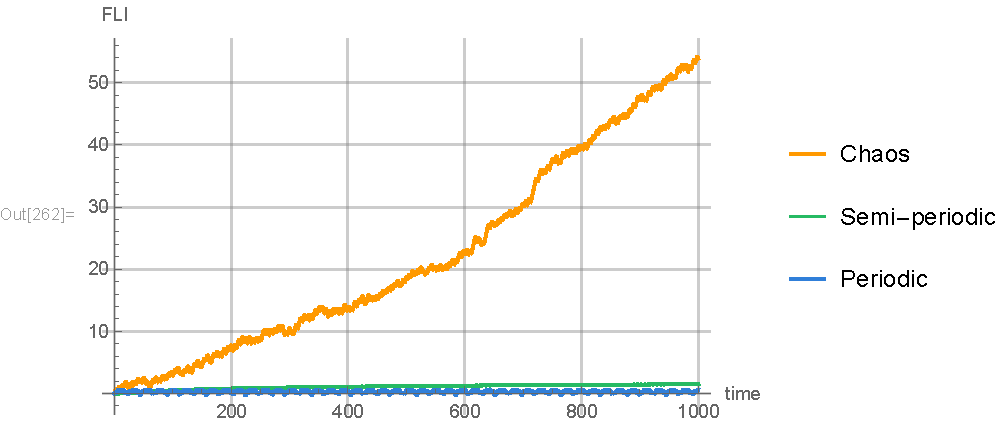
\includegraphics{AD_Pend_4/FLI_time.pdf}
    \caption{Δείκτης \textlatin{FLI} συναρτήσει του χρόνου}
    \label{fig:fli_index}
\end{figure}

Παρατηρούμε πως ο δείκτης \textlatin{FLI} για την χαοτική τροχιά αυξάνει με γραμμικό τρόπο, ενώ για την ημιπεριοδική και την περιοδική τροχιά η αύξηση είναι αρκετά πιο αργή (αυξάνει λογαριθμικά).

\subsection{Ερώτημα Δ}

\indent Υπολογίστε για τις παραπάνω τροχίες τον εκθέτη \textlatin{Lyapunov} (δες παράγραφο 7.6.2) (σε ένα διάγραμμα και για τις τρεις τροχίες).

\subsubsection{Λύση}

\indent Για τον εκθέτη Lyapunov έχουμε τις αρχικές δυο εξισώσεις:

\begin{align}
    \dot{x_1}(t)&=f_1=x_2(t)\\
    \dot{x_2}(t)&=f_2=-\frac{1}{(1+0.1 \sin (3 t))} \sin x_1(t)
\end{align}

Για να βρούμε τις άλλες δύο εξισώσεις θα επιλύσουμε το γραμμικό σύστημα:

\begin{equation}
\left(\begin{array}{l}
\dot{\xi} \\
\dot{\eta}
\end{array}\right)=\left(\begin{array}{ll}
\frac{\partial f_{1}}{\partial x} & \frac{\partial f_{1}}{\partial y} \\
\frac{\partial f_{2}}{\partial x} & \frac{\partial f_{2}}{\partial y}
\end{array}\right)_{0}\left(\begin{array}{l}
\xi \\
\eta
\end{array}\right)
\end{equation}

Το οποίο τελικά θα μας δώσεις τις δύο τελευταίες εξισώσεις:

\begin{align}
    \dot{\xi}&=\eta\\
    \dot{\eta}&=-\frac{\cos{x_1(t)}}{1+0.1\sin{3t}}
\end{align}

Οπότε έχουμε τις απαιτούμενες εξισώσεις για να υπολογίσουμε τον εκθέτη \textlatin{Lyapunov}, και συγκεκριμένα τον χαρακτηριστικό αριθμό \textlatin{Lyapunov}. Τρέχουμε το πρόγραμμα τρεις φορές για κάθε μια περίπτωση, αυξάνοντας τον χρόνο ολοκλήρωσης σε \(t_{max}=10000\). 

\begin{figure}[H]
    \centering
    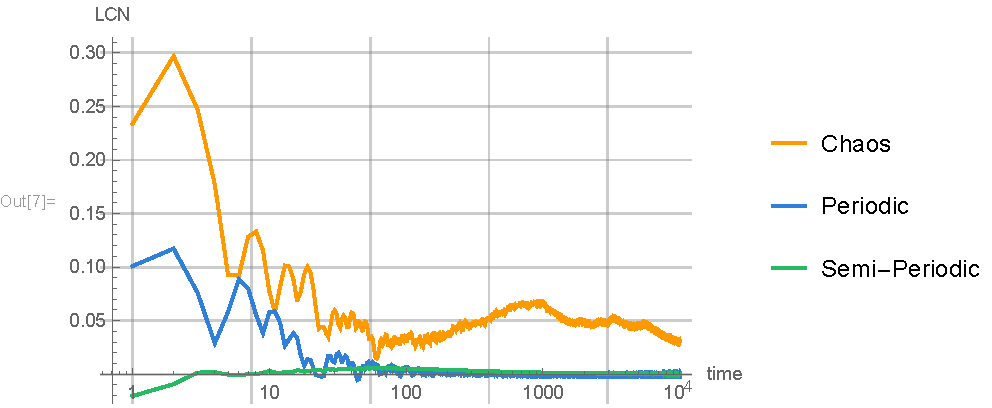
\includegraphics{AD_Pend_4/LCN_combined.pdf}
    \caption{\textlatin{LCN} συναρτήσει του χρόνου}
    \label{fig:LCN_combined}
\end{figure}

Παρατηρούμε πως ο χαρακτηριστικός αριθμός \textlatin{Lyapunov} για την περιοδική και την ημιπεριοδική τροχιά τείνουν γρήγορα προς το μηδεν και παραμένουν πρακτικά μηδενικοί για μεγαλύτερους χρόνους, επιβεβαιώνοντας πως έχουμε να κάνουμε με κανονικές τροχίες. Αντιθέτως, ο χαρακτηριστικός αριθμός \textlatin{Lyapunov} για την χαοτική τροχιά δεν φαίνεται να μηδενίζεται και για μεγαλύτερους χρόνους ολοκλήρωσης θα τείνει σε μια σταθερή τιμή.

\subsection{Ερώτημα Ε}

\indent Υπάρχουν τροχίες κατά τις οποίες το εκκρεμές ταλαντώνεται γύρω από γωνία \(\theta \neq 0\)? Αν ναι, δώστε τις αρχικές συνθήκες και σχεδιάστε την ταλάντωση \(\theta=\theta(t)\) για ένα ενδεικτικό διάστημα.

\subsubsection{Λύση}

\indent Δεν εντοπίστηκαν τροχιές για τις οποίες το εκκρεμές ταλαντώνονται σε γωνία διαφορετική του μηδενός.

\subsection{Ερώτημα ΣΤ}

\indent Όπως στο ερώτημα Β (αλλά με λιγότερες αρχικές συνθήκες) σχεδιάστε την απεικόνιση \textlatin{Poincare} για συχνότητα εξωτερικής διέγερσης 10πλάσια αυτής που δίνεται. Τι παρατηρείτε για τη χαοτική ζώνη γύρω από το σημείο \(\theta=\pi\)?

\subsubsection{Λύση}

\indent Αρχικά θα δείξουμε την τομή \textlatin{Poincare} για αρχικές συνθήκες \(\theta=\pi\) και \(\dot{\theta}=0\):

\begin{figure}[H]
    \centering
    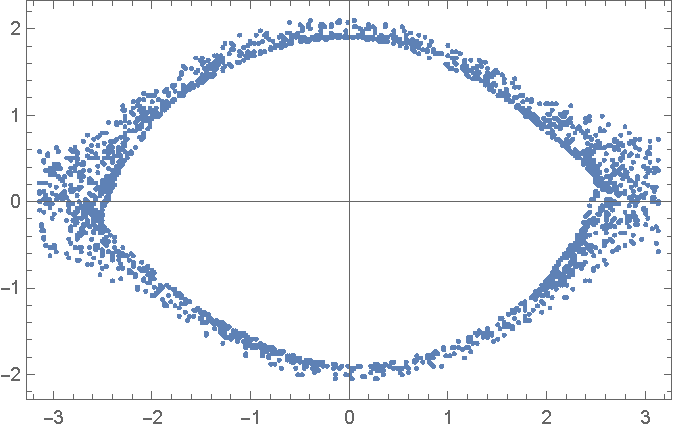
\includegraphics{AD_Pend_4/poincare_pi_initial.pdf}
    \caption{Τομή \textlatin{Poincare} για \(\omega=3\) \((\theta=\pi,\;\dot{\theta}=0)\)}
    \label{fig:initial_poincare}
\end{figure}

Αυξάνουμε τώρα την συχνότητα σε \(\omega=30\) και σχεδιάζουμε εκ νέου την τομή \textlatin{Poincare}:

\begin{figure}[H]
    \centering
    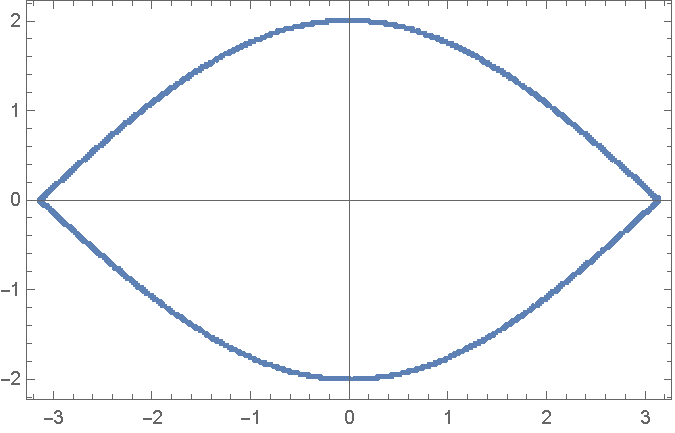
\includegraphics{AD_Pend_4/poincare_pi_final.pdf}
    \caption{Τομή \textlatin{Poincare} για \(\omega=30\) \((\theta=\pi,\;\dot{\theta}=0) \) }
    \label{fig:final_poincare}
\end{figure}

Παρατηρούμε πως με την αύξηση της συχνότητας η χαοτική συμπεριφορά εξαφανίζεται και δίνει τη θέσης της σε μια ημιπεριοδική τροχιά. Το συμπέρασμα αυτό επιβεβαιώνεται και μέσω του δείκτη \textlatin{FLI} ο οποίος τώρα αυξάνει για τα πρώτα χρονικά βήματα αλλά στη συνέχεια παραμένει σταθερός και δεν παρατηρείται περαιτέρω αύξηση, η οποία είναι χαρακτηριστική της χαοτικής συμπεριφοράς.

\end{document}